% Template for PLoS
% Version 1.0 January 2009
%
% To compile to pdf, run:
% latex plos.template
% bibtex plos.template
% latex plos.template
% latex plos.template
% dvipdf plos.template

\documentclass[10pt]{article}

% amsmath package, useful for mathematical formulas
\usepackage{amsmath}
% amssymb package, useful for mathematical symbols
\usepackage{amssymb}

% graphicx package, useful for including eps and pdf graphics
% include graphics with the command \includegraphics
\usepackage{graphicx}

% cite package, to clean up citations in the main text. Do not remove.
\usepackage{cite}

\usepackage{color} 



% Use doublespacing - comment out for single spacing
%\usepackage{setspace} 
%\doublespacing


% Text layout
\topmargin 0.0cm
\oddsidemargin 0.5cm
\evensidemargin 0.5cm
\textwidth 16cm 
\textheight 21cm

% Bold the 'Figure #' in the caption and separate it with a period
% Captions will be left justified
\usepackage[labelfont=bf,labelsep=period,justification=raggedright]{caption}

% Use the PLoS provided bibtex style
\bibliographystyle{plos2009}

% Remove brackets from numbering in List of References
\makeatletter
\renewcommand{\@biblabel}[1]{\quad#1.}
\makeatother


% Leave date blank
\date{}

\pagestyle{myheadings}
%% ** EDIT HERE **


%% ** EDIT HERE **
%% PLEASE INCLUDE ALL MACROS BELOW

%% END MACROS SECTION

\begin{document}

% Title must be 150 characters or less
\begin{flushleft}
{\Large
\textbf{Strive or Collapse: How Cooperative Societies Face Property Violations}}
% Insert Author names, affiliations and corresponding author email.
\\
Author1$^{1}$, 
Author2$^{2}$, 
Author3$^{3,\ast}$
\\
\bf{1} Author1 Dept/Program/Center, Institution Name, City, State, Country
\\
\bf{2} Author2 Dept/Program/Center, Institution Name, City, State, Country
\\
\bf{3} Author3 Dept/Program/Center, Institution Name, City, State, Country
\\
$\ast$ E-mail: Corresponding maillart@berkeley.edu
\end{flushleft}

% Please keep the abstract between 250 and 300 words
\section*{Abstract}

According to John Locke (1689) ``The reason why men enter into society, is the preservation of their property [...] to limit the power, and moderate the dominion, of every part and member of the society.
" \cite{locke2014second}: As long as property violations and enduring costs remain marginal, people can 
engage into trustworthy contractual business relationships, which in turn bring individual and collective wealth \cite{}. Despite the importance of property rights and its implication \cite{}, it remains unclear by which mechanisms property right violations undermine cooperative societies in which individuals can choose their strategies in a prisoner's dilemma game with neighbors (cooperate or defect), and can migrate either to empty locations, or by expelling other individuals from their location. While little property violation may be beneficial for cooperation (in particular for small migration ranges), beyond a threshold is not sustainable: The more property violation the more cooperation is likely to collapse (this threshold is controlled by population density and migration range cooperation). We find that cooperation may be maintained only if the payoff from {\it prisoner's dilemma update} remains smaller than the payoff resulting from {\it success-driven migration} or from {\it property violation}. In that case, payoffs from available strategies (prisoner's dilemma update, success-driven migration, property violation) get decoupled and reach stationarity, ensuring long-term cooperation, while strongly coupled strategies lead to the collapse of cooperation. When cooperation is sustained, migration ranges for success-driven migration and property violation remain rather small (regardless of the migration range), showing that mitigation of property violators is best achieved {\it locally}. If a population is already organized against property violators, it can in fact cope with up to 20\% more property violation than the maximum level at which it achieved enduring organization.
  
%\section*{Author Summary}

%\section*{Introduction}
\clearpage

\section*{Introduction}
The protection of private property counts among the oldest \cite{benson1989enforcement} and the most pervasive social norms and legal provisions across societies \cite{sened1997political}. Likewise, numbers of living systems have developed strategies to protect against foreign invaders as well as insider threats (e.g. the immune system), in order to ensure exclusive consumptions of resources and maintain homeostasis among constituting components of organisms \cite{}. In human systems, John Locke posited the very existence of societies by individuals seeking protection for their private property \cite{locke2014second}. The protection of private property may be ensured by fostering cooperation and trust through social norms, emerging in endogenous fashions among individuals, hence reducing free-riding among individuals \cite{}. Property enforcement may also be brought by exogenous rules elaborated by institutions representing a collective social endeavor (Efficient institutions for the private enforcement of law \cite{friedman1984efficient}).\\


{\bf[sideline thought :]}For example, in capitalist economies, labor unions bring employees together in order to balance the power of employers, and to ensure that privileges are fairly distributed among all workers \cite{}; International organizations and international treaties aim to reduce the preponderant influence of powerful states. Even with highly cooperative institutions based on sharing resources, such as the commons, rules are implemented to ensure that individual rights are respected \cite{ostrom1990governing}. \\

{\bf [some sideline citations:]}
{\it The origin of the family, private property and the state} \cite{engels1978origin}. {\it The exchange and enforcement of property rights} \cite{demsetz1964exchange}. {\it The boundaries of private property: how shall private property be divided: legal and constitutional challenges in such regulations} \cite{heller1999boundaries}\\

This study is motivated by the observation that the individual property rights are precious and thus regularly challenged in a number of ways, including attempts to overtake real-estate \cite{anderson1975evolution}, human rights \cite{}, privacy \cite{warren1890right} and digital privacy \cite{acquisti2013privacy}. Successful abuses of property rights make the violator better off and leave the incumbent abused individual in a less favorable situation. For example, in case of real-estate property violation, the incumbent may suffer some negative utility and in the worst case might be forced to find another location to settle. Unless they are themselves aimed at the systematic abuse of individual rights, governments are concerned by individual property right violations, as property crime may undermine trust and cooperation between individuals. In turn, trust and cooperation help keep defection and abuse at bay \cite{}, although it has been found that some level of free-riding actually help establish and maintain cooperation \cite{}. One contemporary instance of individual property violation is (online) identity fraud, which may undermine trust in online commerce, online administration and more generally exchange of information \cite{}.\\

Unlike other systems (e.g. markets?), which may converge to a social optimal stable equilibrium, fixing the ``right" level of private property enforcement (and hence an affordable level of property crime) through self-organized social norms or through institutions has remained a complicated problem: Because property law enforcement may become intrusive and thus undermine the trust in the law enforcement institution (think of government surveillance) \cite{johnsongovernment}, people desire the strict minimum amount property enforcement required to maintain a cooperative society . Also, going back to Locke, the very action of entering society represents by itself the alienation of a substantial portion of ``libre arbitre". Additionally, property crime enforcement by an institution is a costly business (find figures?), which shall consume as little as possible resources. There is thus a natural incentive to determine and to fix the maximum level of property violation (resp. the minimum level of private property enforcement) beyond (resp. below) which cooperation and trust are in danger of collapse.\\

Here, we question the nature of the maximum affordable level of property violation beyond which society is no longer sustainable, and considering that this optimal point shall not be found at once (i.e., {\it ex-ante} when a society is trying to get estalished), we shall investigate when and how much corrective actions shall be taken to restore high levels of trust and cooperation before it becomes too late.\\

For that purpose, we consider a public goods ``trust" game,\cite{} in which individuals play the prisoners' dilemma with their neighbors, and may move within a migration range to empty locations (i.e., success-driven migration) or on the contrary to occupied locations (i.e. property violation), forcing the incumbent individual to move to the next best empty site.\\

Recent work in game theory has shown that success-driven migration enhances and even elicits the outbreak of cooperation in the presence of combined imitation + mobility randomness \cite{helbing2009outbreak}, while most previous studies found that mobility can undermine cooperation by supporting defector invasion \cite{}. \\ %The conditions under which cooperation is maintained have extensively studied \cite{}, including with mobility \cite{} and randomness \cite{}. \\

Property violation forces to consider the effects of migration in an original fashion, where randomness stems from the probability by a player to take over the more favorable location of another individual. The property violation level reflects the expected success of property violation given all means deployed by society to prevent it as an equilibrium of forces between property violations capabilities on the one hand, and property enforcement on the other hand.\\

Property violation is also highly related to density and migration range {\bf [bring  more context here $\rightarrow$ Maybe in The evolution of property rights: a study of the American West \cite{anderson1975evolution};The private enforcement of law \cite{landes1974private}]}. Say something on density versus crime.\\



\section*{Private Property Model}
Our study is carried out for the prisoner's dilemma game (PD), which is often used to model selfish behavior of individuals when cooperation is risky and defection is tempting, but where the outcome of mutual defection is inferior to cooperation on both sides \cite{axelrod1981evolution,nowak2006five}. 
Formally, the so-called reward $R$ represents the payoff for mutual cooperation, while the payoff for defection of both sides is the {\it punishment} $P$. $T$ represents the {\it temptation} to unilaterally defect, which results in the {\it sucker's payoff} $S$ for the cooperating individual. The inequalities $T > R > P > S$ and $2R > T + S$ define the classical prisoner's dilemma, in which it is more profitable to defect, no matter what strategy the other individual selects. Therefore, rationally behaving individuals would be expected to defect when they meet once. However, defection by everyone is implied as well by the game-dynamical replicator equation \cite{epstein1998zones}, which takes into account imitation of superior strategies, or payoff-driven birth-and-death processes. In contrast, a coexistence of cooperators and defectors is predicted for the snowdrift game (SD). Although it is also used to study social cooperation, its payoffs are characterized by $T > R > S > P$ (i.e., $S > P$ rather than $P > S$) \cite{}.\\

As is well-known \cite{nowak2006five}, cooperation can, for example, be supported by repeated interactions \cite{axelrod1981evolution}, by intergroup competition with or without altruistic punishment\cite{traulsen2006evolution,fehr2002altruistic,boyd2003evolution}, and by network reciprocity based on the clustering of cooperators \cite{nowak1992evolutionary,szabo2002phase,hauert2004spatial}. In the latter case, the level of cooperation in 2-dimensional spatial games is further enhanced by ``disordered environments" (10\% inaccessible empty locations) \cite{vainstein2001disordered}, and by
diffusive mobility, provided that the mobility parameter is in a suitable range \cite{vainstein2007does}. Usually, strategy mutations, random relocations, and other sources of stochasticity can significantly challenge the formation and survival of cooperative clusters \cite{}. {\it Success-driven} migration, in contrast, is a robust mechanism: By leaving unfavorable neighborhoods, seeking more favorable
ones, and remaining in cooperative neighborhoods, it supports cooperative clusters very efficiently against the destructive effects of noise, thus preventing defector invasion in a large area of payoff parameters \cite{helbing2009outbreak}.\\

The {\it private property} game implies the possibility to expel players from locations with higher pay-off, and as such, it extends the success-driven migration game by allowing migrations to any location within the migration range. We assume $N$ individuals on a two dimension square with periodic boundary conditions and $L\times L$ sites, which are either empty or occupied by one individual. Population density $d$ is a parameter with values between $0.2$ and $0.8$.\footnote{below and beyond these values, a migration game makes little sense as interactions in low density worlds may only be achievedby large migration ranges, and densities $\rightarrow 1$ almost completely remove migration opportunities.} Individuals are updated asynchronously, in a random sequential order, and each individual gets updated on average $N$ times (i.e., the number of Monte Carlo Steps $MCS = N \times L^2$). At each step, the randomly selected individual performs simultaneous interactions with the $4$ direct neighbors and compares the overall payoff with that of these neighbors. If one neighbor has a better payoff, the individual updates her strategy with the one of her best performing neighbor.\footnote{Performing the same simulations with 8 neighbors does not change the picture overall.} In absence of noise ($r=0$, equiv Fermi temperature equals to 1), this update is sure, and the individual cannot spontaneously start to cooperate ($q=0$).\\

The migration step is performed before the imitation step\cite{helbing2009outbreak}: An individual explores the expected payoffs for {\it all} sites in the Moore neighborhood $(2M + 1) \times (2M + 1)$ of range $M$. If the fictitious payoff is higher than in the current location, the individual is assumed to move to the site with the highest payoff with probability $m$ (in absence of migration noise, $m=1$). If the target site is empty, then {\it success-driven} migration occurs. On the contrary, if the site with highest payoff is already occupied by another individual, the {\it property-violation} migration occurs. With probability $s$, the focal player takes the site of the incumbent individual, who in turn is expelled to the best empty site in her own Moore neighborhood (see Figure \ref{fig:migration_diagram} for a graphical representation). With probability $1-s$ however, property violation is aborted and the individual migrates to the best empty site within the migration range. The probability $s$ encompasses the unsure nature of the property violation endeavor such as the possibility to get caught by law enforcement, or limited by some physical or technical constraints. \\
 
While small quantities of property violation introduce some amount of randomness that enhances cooperation (see Figure \ref{fig:phase_transition}a), our model is aimed at uncovering the limit conditions and the mechanisms, which help maintain or restore cooperative societies in presence of property violation. Indeed, it makes particularly sense to study limit conditions in the case of private property violation, because society want to optimize their law enforcement, hence invest the minimum for the maximum effects.\footnote{Here, we can enrich the paragraph by pulling out complex system research on transition from order to disorder (and vice-versa) when a system is optimized.}

%The resulting strategy mutations reflect deficient imitation or trial-and-error behavior. As a side effect, such noise leads to an independence of the final cooperation level from the initial one (at $t=0$), and a {\it qualitatively different} pattern formation dynamics for the same payoff values, update rules, and initial conditions ( c.f. SI Fig.1). Using the alternative Fermi update rule \cite{} would have been possible as well. However, resetting strategies rather than inverting them, combined with values $q$ much smaller than $0.5$, creates particularly adverse conditions for cooperation.\\



\section*{Results}
Computer simulations of the model presented above show that the probability of property violation $s^{*}$ beyond which cooperation cannot not survive is highly dependent on the migration range $M$ and the population density $d$. At time $t=0$, the simulation starts with an equiprobable number of cooperators and defectors scattered uniformly across occupied sites.\\ 

When there is no migration ($M=0$), and by definition no property violation ($s=0$), evolution occurs only through replication of direct neighbor strategies. Cooperators form clusters to prevent invasion by defectors (see Figure \ref{fig:configurations_t200}{\it A}). In absence of property violation, any migration range $M \geqslant 1$ unambiguously promotes cooperation (see for instance Figures \ref{fig:configurations_t200}{\it B} and \ref{fig:configurations_t200}{\it E}, and defectors rapidly disappear (the migration range has no effect on the speed at which cooperators invade the population. See Figure SI \ref{figSI}).\\

However, considering the evolution of cooperation when individuals have small migration range $M \leqslant 5$, even little property violation can completely destroy cooperation, past an abrupt critical (phase transition) point $s^{*}$. For instance, for a unit Moore's migration range, a $8\%$ probability property violation is sufficient to destroy cooperation (see Figure \ref{fig:configurations_t200}{\it D}, as well as Figure \ref{fig:configurations_t200}{\it G} for $M=5$). For $s < s^{*}$, a majority of cooperators ($c>0.5$), along with a minority of defectors, which cluster together for $M=1$ (see Figure \ref{fig:configurations_t200}{\it C}) or scatter around clusters of cooperators for $M \geqslant 5$ (see e.g., Figure \ref{fig:configurations_t200}{\it F}).\\

With larger Moore migration ranges ($M \geqslant 5$), cooperative populations can sustain much more property violation. For instance, for population density $d=0.5$, cooperators account for on average 80\% of the population after 200 iterations, with property violation as large as $s^{*}_{-} = 0.45$ with migration range $M=11$ (see Figure \ref{fig:configurations_t200_M11plus}{\it B}), as well as for $M=13$ and nearly half chance for property violation (see Figure \ref{fig:configurations_t200_M11plus}{\it F}).\\

Also for large migration ranges ($M \geqslant 5$), an intermediary state $s^{*}_{-} \leqslant s \leqslant s^{*}_{+}$ appears, in which cooperative populations can survive while on average in minority (see Figures \ref{fig:configurations_t200_M11plus}{\it C} and \ref{fig:configurations_t200_M11plus}{\it G}). For $s > s^{*}_{+}$, cooperative populations do not strive (see Figures \ref{fig:configurations_t200_M11plus}{\it D} and \ref{fig:configurations_t200_M11plus}{\it H}).\\

As individuals search their {\it best-shot} -- maximizing expected pay-off at the selected location (in their Moore's migration range $M$) -- they only try to expel another individual, with property violation probability $s$, if this {\it best-shot} location is already occupied. The effects on cooperation, are not only a function of property violation, but also of the migration range as well as the population density: The lower the density $d$ and the larger the migration range $M$, the more opportunities to find a {\it best-shot} location, which is empty. On the contrary, the higher the population density and the smaller the migration range, the more individuals must rely on property violation to make a successful move. As shown on Figure \ref{fig:heatmaps} for $M= \{ 5,7,11,18\}$, the level of property violation $s^{*}$ beyond which cooperation cannot survive, depends on both the migration range $M$ and the population density $s$. For large $M \geqslant  7$, the intermediary state $s^{*}_{-} \leqslant s \leqslant s^{*}_{+}$, where cooperative populations can survive while on average in minority, appears in green. We also find that for high population densities $d > 0.9$, cooperation cannot survive for $s > 0$; Even with no property violation $s=0$, there is a probability that cooperators cannot invade the whole population, in particular for large migration ranges (see SI Section \ref{SI:d09}).\\


\subsection*{Going Further}
To further understand the properties of the {\it property game} as a special {\it success-driven} migration game, we shall consider how individuals exploit the degrees of freedom offered to them, such as empty sites available when $d < 1$ and their capabilities to reach these sites according to their mobility $M > 0$, how they achieve even greater opportunities by expelling individuals from their location. We finally investigate how cooperation is affected by the relocation of expelled individuals. In our model, individuals are fully rational as they will imitate they imitate their neighbors and migrate with probability $1$, if the find a strategy and a location respectively, with higher payoff. Only the probability of property violation is uncertain and controlled by $0 \leqslant s \leqslant 1$. \\

{\bf We consider the actual mobility if individuals $m = \sqrt{|x^2 + y^2|} \leqslant M$ bounded by the migration range $M$, versus average distance of sites (weighted by their payoff and whether they are free or not). This has something to do with the structure of clusters $\rightarrow$ a proxy could be density of cooperators vs. defectors in the migration range}.

{\bf We shall also who uses property violation? defectors or cooperators?}

{\bf Note that the larger the migration range, the more likely to find a number of sites for which the payoff is the same. In that case, the migration site is chosen in the following way: randomly among empty sites, and if there is no empty site, randomly among non empty site with some probability of property violation $s$. Note that calculating payoff from 8 neighbors instead of 4 may help alleviate this intrinsic randomness.}

{\bf Note that if the migration range is large enough, agents can ``jump" from one cluster to another $\rightarrow$  think of hubs (technology, finance, politics)}

%\section*{Discussion}



\subsection*{Limitations}

- What the resource is not exclusive (e.g. personal information)?


\section*{Conclusion}
The {\it property game} exhibits a tipping point, which occurs way before the large-scale effects leading to collapse actually unfold. This mechanism is reminiscent of other global problems, such as climate change, with long delay between the almost unnoticeable mechanism activation leading to collapse, and the actual edge of collapse. Our results show that in the case of private property, the mechanism is reversible, provided that authorities can act very pro-actively at the (little) cost of little correction action, or only with drastic property crime reduction (at high costs) if the problem is tackled after it gets noticed (reduction of cooperation).\footnote{I feel frustrated in the end because I think the message by John Locke was that people would start to cooperate (and form a society as this cooperation goes beyond a one-to-one cooperation) in order to keep private property violators at bay. However, here nothing shows that private property triggers some cooperation at the exception of very small amount of property violation. In future work, we can see the problem in 2 non-exclusive ways: The first solution is a little hand-wavy and considers that cooperation actually increases with a little property violation. Actually, one can ``boot" cooperation with ``only" 30\% cooperators (randomly scattered) at $t=0$ ($d=0.5,M=5$). With more trials, it may be possible to lower this threshold. Starting with small clusters (e.g. like a family) may also help lower the threshold. The second solution is more realistic but also more tricky technically. It consist in considering a cooperative cluster as ``an autonomous society" or at least a autonomous sub-component of an entire society, which may be the scale at which property violation is actually tackled in the decoupled (striving) regime. This ties back to hierarchies in social group sizes  (c.f., Dunbar and others), as well as the notion of private property in family (c.f. The origin of the family, private property and the state \cite{engels1978origin}?).We could explore this path, but (i) better visualization is needed to get more hints of what's going on, and (ii) one must develop a way to account for the size of these clusters and/or what is special about them. In my mind both ideas are not mutually exclusive: the first is more related to the organization process starting from random organization and the second is more how stability is established and ensured on the long term. We could imagine a way to boot cooperation in adverse conditions (which include property violation) and get cooperation going once clusters are established.}

% Results and Discussion can be combined.

% You may title this section "Methods" or "Models". 
% "Models" is not a valid title for PLoS ONE authors. However, PLoS ONE
% authors may use "Analysis" 
%\section*{Materials and Methods}

% Do NOT remove this, even if you are not including acknowledgments
%\section*{Acknowledgments}


%\section*{References}
% The bibtex filename
\bibliography{../bib/pgame}

\clearpage
\section*{Figures}


\begin{figure}[h]
\begin{center}
\centerline{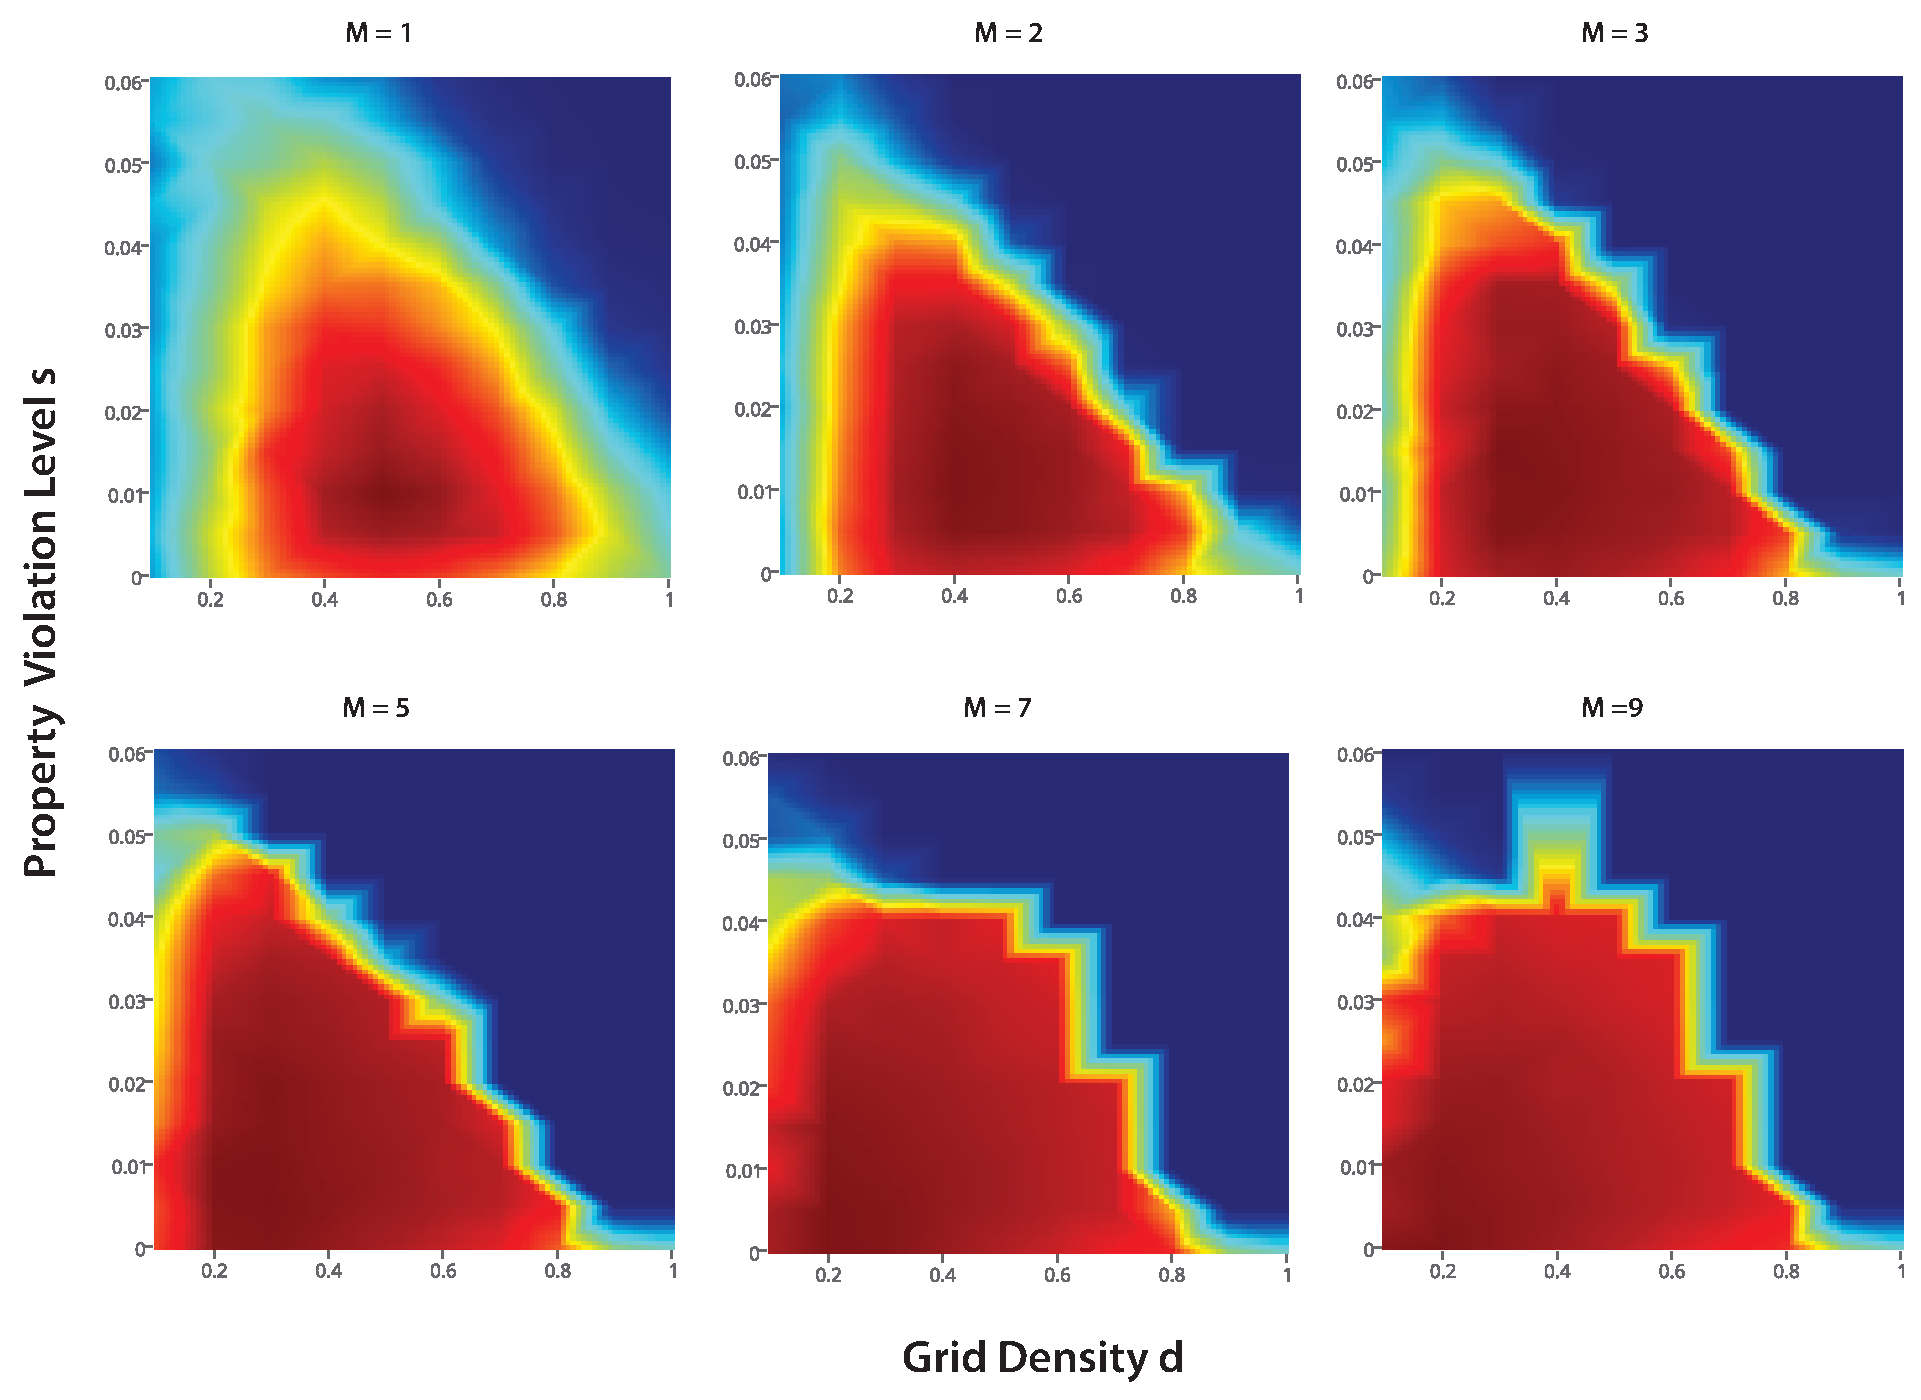
\includegraphics[width=14cm]{../figures2/heatmaps.eps}}
\caption{Cooperation levels after $N=200$ iterations [i.e., $200 \times 49^2 = 480,200$ Monte Carlo Steps (MCS)] for migration Moore's distances $M = \{1,2,3,5,7,9,11,15,20 \}$, as a function of population density $d$ and probability of property violation $s$. At initialization ($t=0$), there is a $50\%$ chance that a player will cooperate (resp. defect). The uneven landscapes reflect the statistical fluctuations of simulations. For all values of $M$, the cooperation exhibits a sharp drop for $d > d^*$  and $s > s^*$ with $(d^*,s^*)$ being a function of $M$. For high grid density ($d > 0.9$), cooperation cannot be sustained even with low property violation. As the migration range gets large $M > 9$ , the area of sustainable cooperation shrinks drastically.%(see SI Section \ref{SI:d09} for further details on {\it migration} and {\it property} games in densely populated worlds).
}
\label{fig:heatmaps}
\end{center}
\end{figure}



\begin{figure}[h]
\begin{center}
\centerline{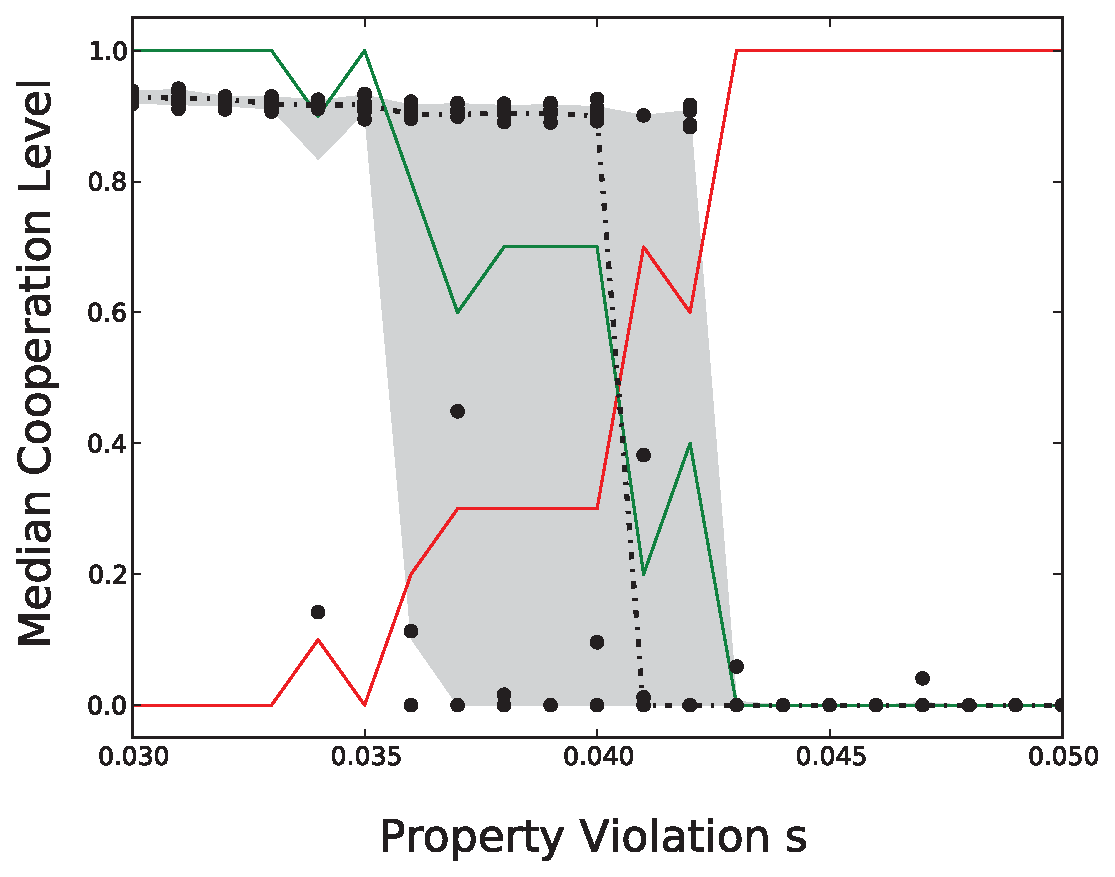
\includegraphics[width=9cm]{../figures2/phase_transition_d05_paper.eps}}
\caption{Phase transition of cooperation levels after $N=200$ iterations [i.e., $200 \times 100^2 = 2M$ Monte Carlo Steps (MCS)] for migration Moore's distance $M = 5$ and population density $d=0.5$. The cooperation level (dotted black line) exhibits a sharp drop around $0.035 < s^{*} < 0.044$, with an equal probability that cooperative players will strive or disappear around $s^{*} \approx 4.01\times10^{-2}$: Probabilities that cooperative players invade the grid ($> 0.8$) or disappears ($< 0.2$) are shown (green and red lines). The cooperation is stochastic and does not depend on the initial grid configuration}
\label{fig:comparison_no_with_migration}
\end{center}
\end{figure}




%\begin{figure}[h]
%\begin{center}
%\centerline{\includegraphics[width=9cm]{../figures/configurations_t200.eps}}
%\caption{Grid configurations at $t=200$, with fully rational agents (probability of imitation $m=1$), and grid density $d=0.5$. When there is no migration $M=0$ (and {\it a fortiori} no property violation $s=0$) (see {\it A.}), clusters of cooperators can only form by local influence, and the simulation is quickly frozen. As the migration range increases, larger clusters form when cooperators (see {\it B.,E.}) or defectors (see {\it D.,G.}) win. At the lower limit of the phase transition point $s \rightarrow s^{*}_{-}$, cooperators form clusters, which stay strong (large?) enough to keep defectors at bay (see {\it C.,F.}). When $s > s^{*}_{+}$ cooperation cannot survive. However, with larger migration range $M=5$, the transition point $s^*$ is almost three times larger, compared to $M=1$.}
%\label{fig:configurations_t200}
%\end{center}
%\end{figure}
%
%
%\begin{figure}[h]
%\begin{center}
%\centerline{\includegraphics[width=11cm]{../figures/configurations_t200_M11plus.eps}}
%\caption{Grid configurations at $t=200$, with fully rational agents (probability of imitation $m=1$), and grid density $d=0.5$ in the case of large migration ranges ($M = \{11,13\}$). For $M$ large enough, two distinct transition points appear ($s^{*}_{-}$ and $s^{*}_{+}$), with an intermediary stable state (see {\it C.} and {\it G.}), where cooperators are in minority ($c = 0.45\pm0.05$), yet their clusters resistant to defector invasions. Note that configurations look the same for $M=11$ and $M=13$, but the transition interval $(s^{*}_{-}$,$s^{*}_{+}$ has slightly larger values in the latter case, suggesting that populations with larger migration range can sustain more property violation.}
%\label{fig:configurations_t200_M11plus}
%\end{center}
%\end{figure}


%\begin{figure}[h]
%\begin{center}
%\centerline{\includegraphics[width=11cm]{../figures/configurations_t200.eps}}
%\caption{Grid configurations at $t=200$, with fully rational agents (probability of imitation $m=1$), and grid density $d=0.5$. When no migration (and {\it a fortiori} no property violation) is present (see {\it A.}), clusters of cooperators can only form by local influence, and the simulation is quickly frozen. As the migration range increases,  larger clusters form when cooperators (see {\it B.,E.}) or defectors (see {\it D.,G.}) win. At the lower limit of the phase transition point $s \rightarrow s^{*}_{-}$, cooperators form clusters, which stay strong (large?) enough to keep defectors at bay (see {\it C.,F.}).}\label{fig:comparison_no_with_migration}
%\end{center}
%\end{figure}




%\begin{figure}[h]
%\begin{center}
%\centerline{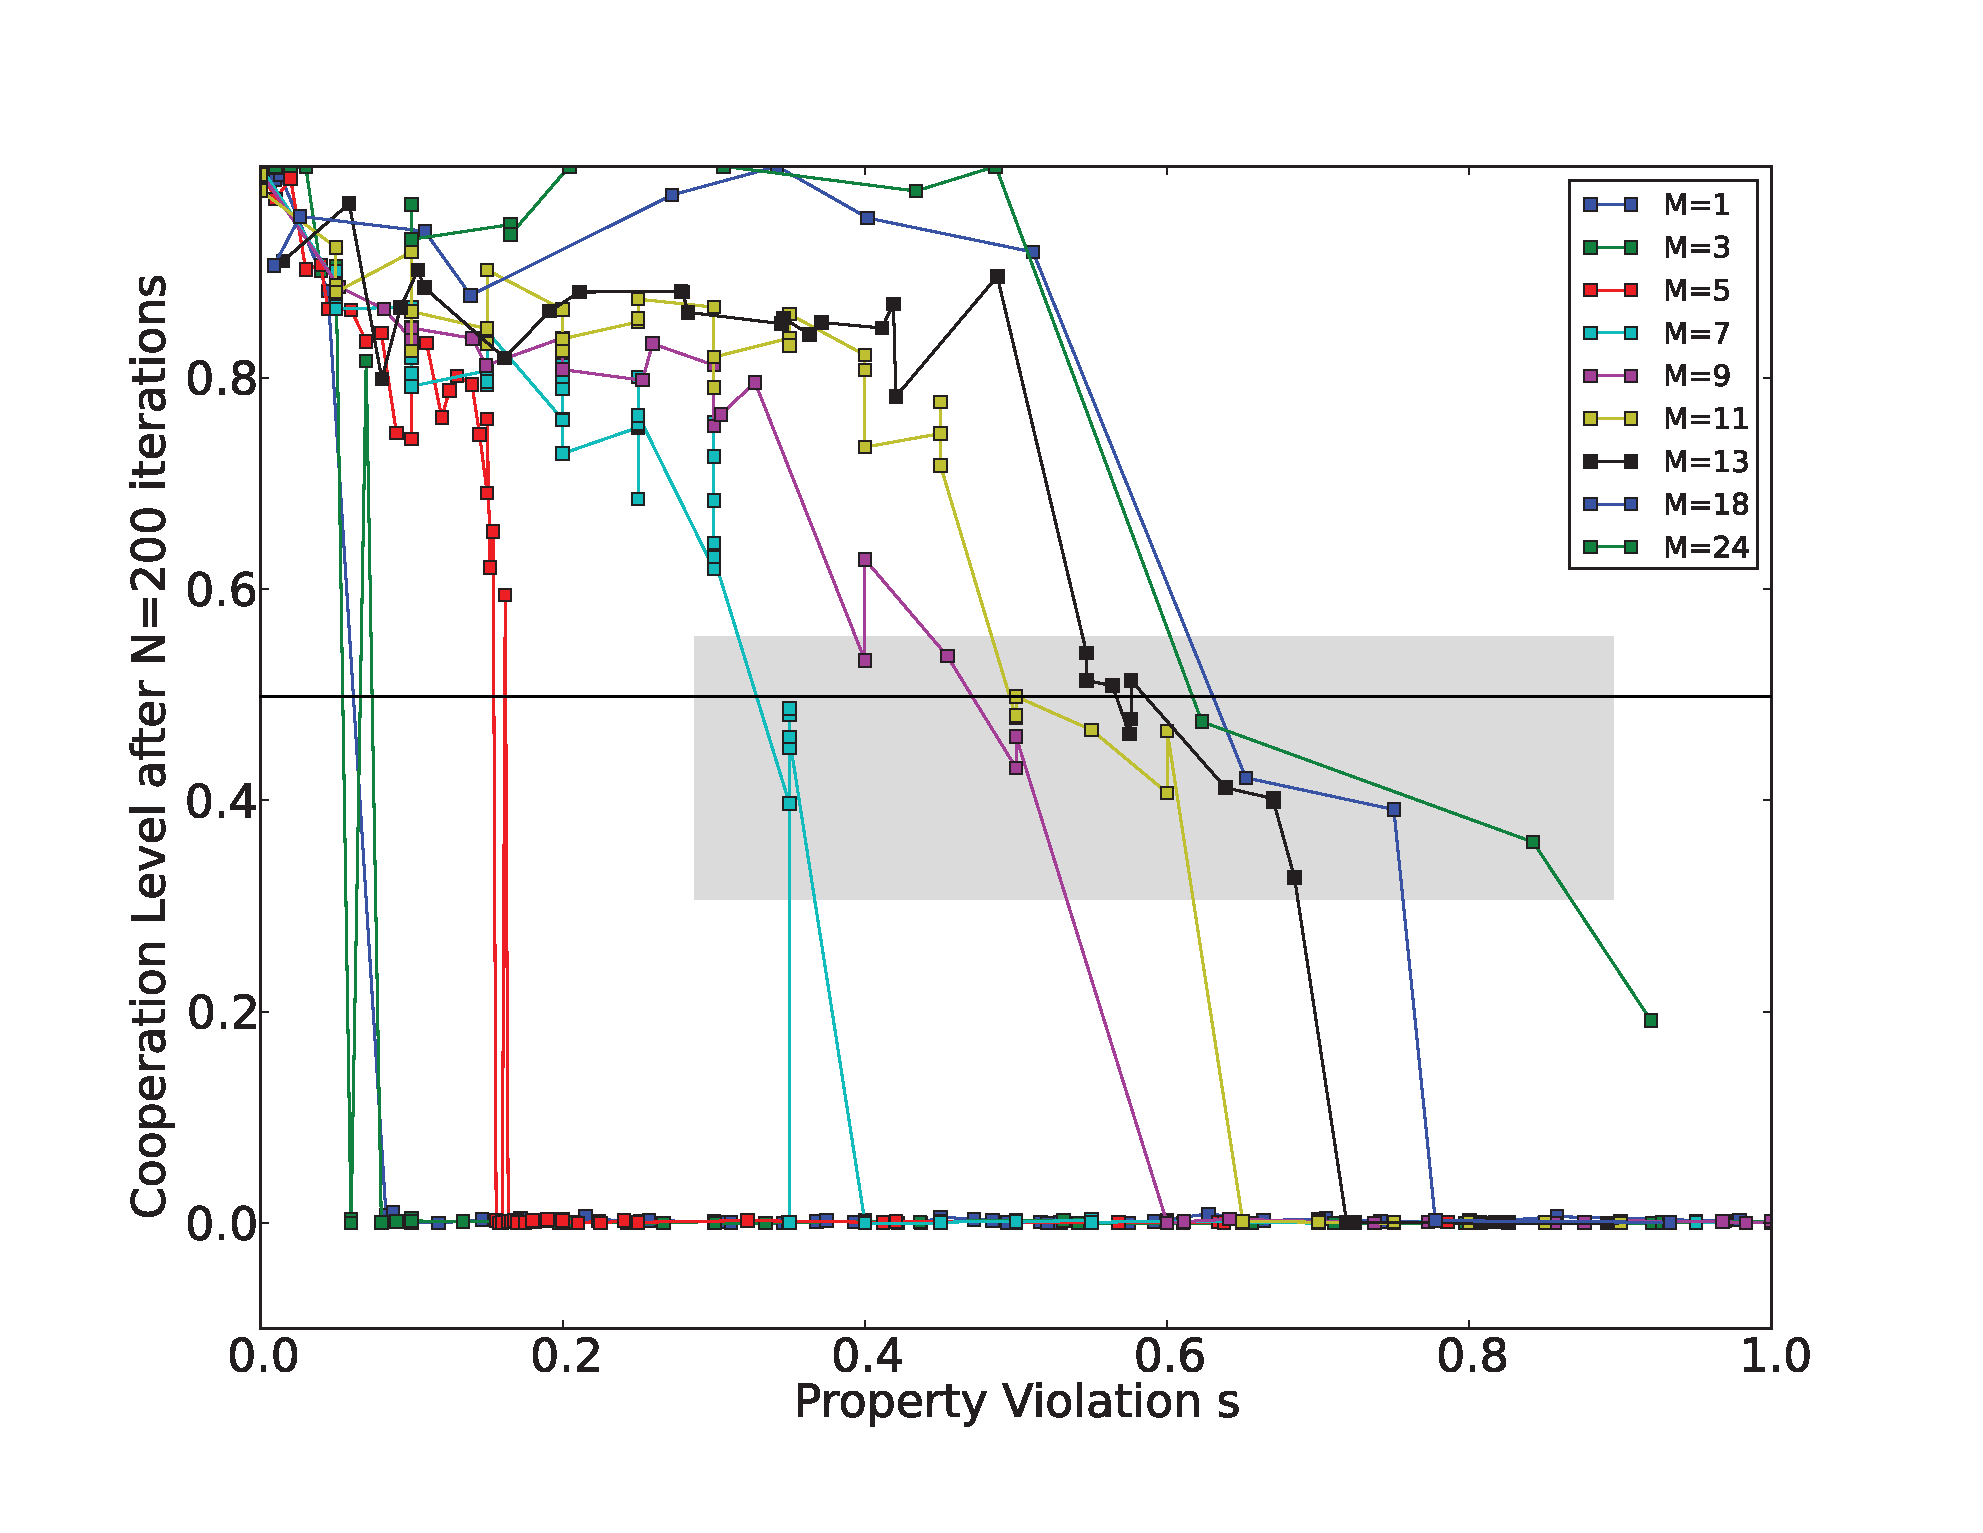
\includegraphics[width=15cm]{../figures/phase_transitions_2.eps}}
%\caption{Typical phase transitions for migration ranges $1 \leqslant M \leqslant 24$ ($0.4 \leqslant d < 0.6$). When there is no property violation $s = 0$, cooperators invade the world for any migration range $M > 0$. For small $M = \{ 1,3,5\}$, a sharp phase transition occurs at a transition point $s^{*}$, from a high level of cooperators in the populations ($c > 0.6$) when $s < s^{*}$ to entire collapse of cooperators for $s > s^{*}$. For $M \leqslant 5$, there is no intermediary state, whereas for $M \geqslant 7$, an intermediary state appears defined by $s^{*}_{-} < s < s^{*}_{+}$, with populations of cooperators in minority ($c \approx 0.45 < 0.5$) compared to defectors. For $M= \{ 7,9\}$, there is a non-zero probability of cooperation collapse, while for larger migration ranges ($M \geqslant 11$), this intermediary state becomes more stable, i.e., process converges almost surely  {\bf [to be further checked]}. Larger migration ranges increase both the maximum number of cooperators when $0 < s < s^{*}_{-}$, increase the lower $s^{*}_{-}$ and higher $s^{*}_{+}$ bounds of property violations, below (resp. above) which cooperative populations win (resp. disappear), and decreases the minimum average proportion of cooperative populations needed in order for cooperation to strive {\bf [to be further checked]}.}
%\label{fig:phase_transition}
%\end{center}
%\end{figure}








%
%
%\begin{figure}[h]
%\begin{center}
%%\centerline{\includegraphics[width=12cm]{Figures/CCDF_A.eps}}
%\caption{Representative spatial organizations for the {\it property game}: {\bf a.} Cooperation can be maintained despite 20\% of property violation probability $(M,d,s) = (9,0.5,0.2)$, {\bf b.} Cooperation collapses quickly for $s>s^*$  $(M,d,s) = (5,0.5,0.5)$, {\bf c.} and {\bf d.} phase transition at $s^{*} = 0.155\pm0.5$ and cooperation can be maintained or on the contrary collapse {\bf [discuss how it may be only a question of time before collapse $\rightarrow$ further simulations + stochastic considerations?]}, {\bf e.} Considerations for $(M,d,s) = (1, 0^+,0.5)$ (c.f. upper left panel Figure \ref{fig:cooperation_M}), and {\bf f.} Considerations for $(M,d,s) = (7,0.9,0^+)$.}
%\label{fig:configurations}
%\end{center}
%\end{figure}



%\section*{Tables}
%\begin{table}[!ht]
%\caption{
%\bf{Table title}}
%\begin{tabular}{|c|c|c|}
%table information
%\end{tabular}
%\begin{flushleft}Table caption
%\end{flushleft}
%\label{tab:label}
% \end{table}

\clearpage

%\section*{Supplementary Material}

\subsection*{SI Text}

\subsubsection*{Motivation and Explanation of the Property Violation Game}

At local, regional and global scales, migrations increasingly occur increasingly in uncontrolled ways, with  number of unintended contingencies and challenges for destinations of migration.\\

Likewise, crime and robbery, which aim to destroy or to steal the property of others, relies on fast mobility in neighborhoods, or cities (c.f., gangs in the USA).\\

In the cyberspace, all neighbors are only a few steps away from each others, physically (think of the Internet Protocol (IP) addressing system) or logically through social networks \cite{degree of separation on Facebook}. \\

With unprecedented mobility, invading, destroying or stealing, abusing the assets of people or communities has never been so accessible, leading to concrete consequences for the stability of physical and online societies. According to repeated United Nation reports, mass migration, resulting from wars and climate change, may threaten the stability of long-established societies across the world. Also, for instance, a high crime rate undermines trust among citizen, reduces the enjoyment, and thus often the economic vigor of a city. Similarly, cyber crime and large-scale cyber attacks undermine trust on the cyber space, and thus, its economic potential.\\

Our {\it private-property} model operationalizes the intricate relationship between success-driven migration -- involving an one-sided move perceived as a violation of property by the other side located at a migration distance -- and how it may undermine trust. Trust is characterized by the capability of individuals to engage into cooperation, in a situation where the Nash equilibrium is 0 ( in other words, when both individuals have an individual incentive to defect). The prisoner's dilemma is such a situation where cooperators trust each others.\\

We have tested our model with a variety of parameters, such as population density, migration range, and the probability of property violation, i.e., the probability that an individual may migrate to an occupied site, hence expelling the incumbent individual to another empty location.\\

The rationale for varying the population density stems from the intuition that densely populated areas are more resource intensive (i.e., available resource per individual is more scarce), and thus, in this case, property violation has more negative effects, such as making relocation more difficult for the expelled individual. We indeed found that beyond a given population density (in general when $d > 0.8$), cooperation cannot survive in presence of even the slightest level of property violation.\\

The large span of Moore's migration range, from very local mobility ($M=1$) to levels close to full mobility on the grid (i.e., $M=24$ for a grid of $49\times49$), reflects large inequalities in mobility at local, regional and global scales, also depending on a given environment. For instance, for those having access to the Internet, mobility is unlimited, at least in theory. Also, populations of wealthy social classes can afford traveling nearly all over the world. On the contrary, some individuals have only very limited mobility within a considered environment. The migration range we used shall be viewed as relative to the world under scrutiny: for $M=1$ the individual can only move by $1/24$ of the world size (defined by a grid of size $49\times49$) at each step; for $M=12$, the individual may move within half the size of the world, which is assumed to be uniformly populated. Clusters may form locally but since only one individual can occupy a grid site the density remains overall well distributed, unlike other types of models such as AB models \cite{solomon} in which multiple agents can accumulate on a single site. The migration range applies to all individuals, regardless whether they just migrate to an empty site or if they attempt to expel another player. There is no designated property violator in our model. All individuals may turn property violators based on their payoff opportunity, as well as following their chance to overcome property enforcement.\\

The probability of property violation reflects the limits of property enforcement, whatever the type of enforcement applied, which can be of legal, police and military nature, or as a result of capabilities by individual to protect their own assets. \\


Configurational Analysis of surprises:

\begin{enumerate}
  \item phase transition as a function of $d,M,s$ $\rightarrow$ study actual migration ranges! 
  \item intermediary state with cooperator level steadily $<0.5$
  \item can we ``boot" a world with less than 50\% cooperators with or without property violation? (in particular, show that the game cannot go to a stable state with $c \approx 0.45$ with such initial level?).
  \item high density populations with $s=0$ and $s >0$ 
\end{enumerate}


{\bf In previous research, Helbing and Yu \cite{} have found that We have searched for conter-intuitive situations where property violations would have positive implications for cooperation. So far, we have not found such a result. The intuition for this hypothesis would be that cooperators forced to migrate would create ``unforeseen" situations, which would help spreading cooperation}.

\subsubsection*{Property game step by step: }

\begin{enumerate}
  \item {\bf Player selection: } At each Monte-Carlo Step ($MCS = N \times l \times h$  with $N$ the number of iterations, and $l$ the grid length and $h$ the grid height) a site is selected. If the site is occupied, the {\bf focal player} is selected. Each player is thus expected to be selected $d \times N$ times with $d$ the grid density. 
  
  \item {\bf Success driven migration (exploration) :} With probability $1 - m$, the focal player strategically explores its own migration (Moore) neighborhood $(2M + 1) \times (2M + 1)$ of range $M$, searching for a site with better payoff with her current strategy (either cooperate or defect). To assess for sites with best payoff, the individual plays the prisoner's dilemma with her own strategy and with neighbors for each site within the migration range. For each site assessed, the ``virtual" payoff is computed as the sum of outcomes from playing the prisoner's dilemma with all neighbors.
  
  \item  {\bf Success driven migration (best empty location) :} If among the sites with the highest payoff, some are empty, the player moves to the closest empty site.
  
  \item  {\bf Success driven migration (property violation) :} If there is no empty site among those with highest payoff, the focal player expels the target player with probability $s$. The expelled target player is forced to move to the empty location with highest payoff within her own migration range. The expelled player may find a new empty site with either higher or lower payoff. For both the focal and the target player, in case multiple sites with highest payoff are available, the closest one is automatically selected. If they are at the same distance, one site is randomly chosen among best sites with smallest migration distance.
  
  \item  {\bf Success driven migration (better empty location) :}  If there is no empty site among those with highest payoff and property violation did not occur, the focal player is forced to move to the empty location with higher -- yet not highest -- payoff, with probability $1 - s$.
  
  \item  {\bf Success driven migration (no migration) :} If all empty sites in the migration range have a payoff worse than the incumbent payoff on the focal site, the player does not move.
  
  \item {\bf Random relocation: } With probability $m$, the focal player relocates to a random location either occupied with probability $s$, or to an empty location with probability $1-s$. There is no consideration of random distance in the case of random relocation.
   
 \item {\bf Imitation step :} Whether it has moved or not, the player is allowed to update her strategy (cooperate or defect), by playing the prisoner's dilemma with her neighbors. If one neighbor's strategy leads to a better payoff, the focal player may imitate this strategy with probability $1-r$. With probability $r$, however, her strategy is reset as follows: the player will cooperate with probability $q$ and defect with probability $1-q$. If the (target) player is forced to move after a property violation, she is not allowed to update her strategy (because it is not her turn to play).
\end{enumerate}



\subsubsection*{Biological and social coevolution (pasted from Helbing and Yu 2009)}. 
We certainly believe that there
could be a coevolution of social behavior and genetically determined
(��hard-wired��) behavior, as is discussed, for example, by
Gintis and Bowles in their articles on strong reciprocity and
human sociality (2, 3). However, it is still worthwhile to ask how
and why strong reciprocators (who cooperate and punish noncooperators
even if the probability of future interactions is low)
would be ��born�� in sufficient numbers to induce the cooperation
of self-interested agents.
The aforementioned coevolution can be represented by models
assuming group selection. For example, a group containing
a sufficient number of strong reciprocators would have larger
chances of survival in a world characterized by frequent crises
than a group containing no or a few strong reciprocators.
Although the connections between group selection and success-
driven migration are rather limited, one could argue that
individuals with a stronger tendency to cluster have an advantage
over individuals who have a weak tendency to cluster. Moreover,
one could think that there is something like a coevolution
between the strategies individuals choose and their spatial
organization. However, none of this is ��hard-wired�� or genetically
inherited in our model. All individuals in our model are
assumed to be of the same kind, and they do not learn to behave
differently in the course of time (i.e., their behavioral rules or
strategy choices are not history-dependent).

\subsubsection*{Costly punishment (paste from Helbing and Yu 2009)}
 In our model, individuals do not impose a cost
on defectors, but they evade future interactions with them. In
comparison with staying in the neighborhood of defectors, this
reduces the average payoff of defectors and may be considered
as a particular kind of punishment. Therefore, our model may
eventually contribute to a better understanding of emergent
norms, which increase the probability of individuals to show
certain behaviors, thereby making social interactions more predictable
and successful on average.
Note that punishment by evasion is not costly for cooperators
in our model. However, evasion from defectors would be costly,
if we would introduce transaction or relocation costs in our
model. These costs, however, would not be restricted to cooperators.
Whenever defectors move into the neighborhood of
cooperators, they have to pay relocation costs as well. As the
relocation costs of cooperators for evading defectors and the
relocation costs of defectors following cooperators are basically
the same, introducing relocation costs does not change the
conclusions of our study.

$\rightarrow$  Actually the migration range is an implicit cost of relocation: if $M$ is small relocation costs are high and the larger $M$ the less costly migration.

\subsubsection*{Network reciprocity, partner selection, and reputation. (paste from Helbing and Yu 2009} Our model introduces a mechanism for the self-organization of cooperative
clusters (assortment), which differs from the clustering mechanism
observed in spatial games without migration. Assortment
is known to support cooperation, and it is sometimes referred to
by the terms network reciprocity or graph selection. In fact,
moving to cooperative neighborhoods reminds of partner selection
(i.e., the formation of a friendship network with cooperative
individuals, while discontinuing interactions with defecting individuals).
However, forming links with friends requires a reputation
mechanism and, with this, higher cognitive abilities.
In our model, individuals do not need to recognize whether
they have interacted with an individual before and do not
remember what strategy this individual applied. In fact, individuals
do not seek friends, and have little control regarding which
individuals they stay close to and, therefore, which individuals
they interact with. Their neighborhood can, in fact, change
significantly. Moreover, in our model individuals are always
exposed to their neighbors, i.e., they cannot avoid further
interactions with neighbors who defected in the past, if they do
not migrate (but then, they will usually lose contact to their
��friends�� as well). If an individual decides to migrate, the new
neighbors will be interaction partners, no matter whether they
are happy with this or not. Therefore, success-driven migration makes weaker and less
favorable assumptions for cooperation than partner selection.
Although the latter can be very selective and allows the creation
of an individualized interaction network, migration can only
choose among available neighborhoods, which also means that
one may have to accept the presence of defectors, if there are no
better choices.




%\begin{figure}[h]
%\begin{center}
%\centerline{\includegraphics[width=18cm]{../figures/cooperation_M.eps}}
%\caption{Cooperation levels after $N=200$ iterations [i.e., $200 \times 49^2 = 480200$ Monte Carlo Steps (MCS)] for migration Moore's distances $M = \{1,3,5,7,9,11 \}$, as a function of the grid density $d$ and the probability of property violation $s$. At initialization ($i=0$), there is a $50\%$ chance that a player will be a cooperation (resp. defector). The uneven landscapes reflect the statistical fluctuations of simulations. For all $M$, the cooperation exhibits a sharp drop for $d>d^*$  and $s > s^*$ with $(d^*,s^*)$ being a function of $M$. In general, cooperation is only close to 100\% if $d \approx 0$ (or $d = 0$ ?). For $d>0$, cooperation drop at 90\% at best. For high grid density ($d>0.9$), cooperation cannot be sustained even with low property violation ($s > 0$). In presence of property violation ($s>0$), cooperation is best sustained for $s \gg 0$, $M \geqslant 7$ and for grid densities $0.4 < d < 0.6$. These results suggest that mobility $M \gg 0$ is efficient to reduce the effects of property violation, provided that the grid is sufficiently dense (to allow formation of clusters of cooperation) but not overcrowded, hence preventing players expelled from their site to choose a reasonably good site. In the limit $d=1$, property violation reduces to swapping sites, since the only available site in the Moore area is the one left by the property violator. }
%\label{fig:cooperation_M}
%\end{center}
%\end{figure}


%\subsubsection*{Low Populated Worlds ($0 < d \leqslant 0.2$)}


\subsection*{Migration and Property Games in Densely Populated Worlds ($d \geqslant 0.9$)}
\label{SI:d09}

In the success-driven migration game, a fully populated world ($d=1$) is only feasible when property violation exists ($s > 0$), since an individual willing to move must expel another individual. In absence of property violation ($s=0$), the game only involves updating strategies with no migration. When $d=1$ and $s > 0$, we find that cooperators cannot strive and disappear after less than 15 iterations.\\

In the limit of population density $d \rightarrow 1$, success driven migration with property violation $s > 0$ leads to a systematic collapse of cooperation. However, for highly densely populated worlds (e.g., $d = 0.9$), even without property violation ($s = 0$), while cooperators can resist to defectors, they may however {\bf not} be able to invade completely the grid (actually, they may be stuck at an intermediate level, usually $ 0.4 \leqslant c \leqslant 0.6$). Cooperators successfully strive and invade almost completely the grid with some probability, which deserves further scrutiny (see Figure \ref{fig:d1_09_s0_outcomes} for a comparison of games with $d=1$ and with $d=0.9$ with same initial conditions but different outcomes).\\

\begin{figure}[H]
\begin{center}
%\centerline{\includegraphics[width=13cm]{../figures/configuration_d09_s0.eps}}
\caption{Evolution of cooperation for $M=\{1,5,9\}$ for $d=1$ and for $d=0.9$, starting from the same initial conditions of a focal simulation (bold line) for which cooperation could invade more than $90\%$ of the grid.}
\label{fig:d1_09_s0_outcomes}
\end{center}
\end{figure}

Here, we question whether the ability by cooperators to invade the grid, is determined by the initial conditions, or on the contrary, if this capability is the result of a chaotic process, when individuals randomly take their turn for migration and strategy update as the simulation proceed. We performed the simulations ten times for $M=3$ and $M=5$ with random initial conditions, and we repeated 10 times the simulations with each of the 10 initial conditions generated. We then counted the number of simulations that ended with $c > 0.9$, conditioned on random conditions on the one hand, and on fixed initial conditions on the other hand.\\

For $M=3$ (resp. $M=5$), we find that high cooperation achievement $c > 0.9$ results at XX\%  (resp. XX\%) from the initial conditions, and XX\% (resp. XX \%) from the random strategy and migration updates by individuals. The latter contribution may be seen as an instance of a chaotic process.\\

%same initial conditions. We find that the probability that cooperation will manage to invade the grid is 0.XX (see Figure \ref{fig:d09_s0_chaotic}). To account for varying densities, we repeated the test for $d=0.85$ and $d=0.95$ ({\bf [to be done]}.\\


%\begin{figure}[H]
%\begin{center}
%%\centerline{\includegraphics[width=13cm]{../figures/configuration_d09_s0.eps}}
%\caption{Evolution of cooperation for $M=\{3,5,9\}$ and $d=0.9$, starting from the same initial conditions of a focal simulation (bold line) for which cooperation could invade more than $90\%$ of the grid.}
%\label{fig:d09_s0_chaotic}
%\end{center}
%\end{figure}

\begin{figure}[H]
\begin{center}
\centerline{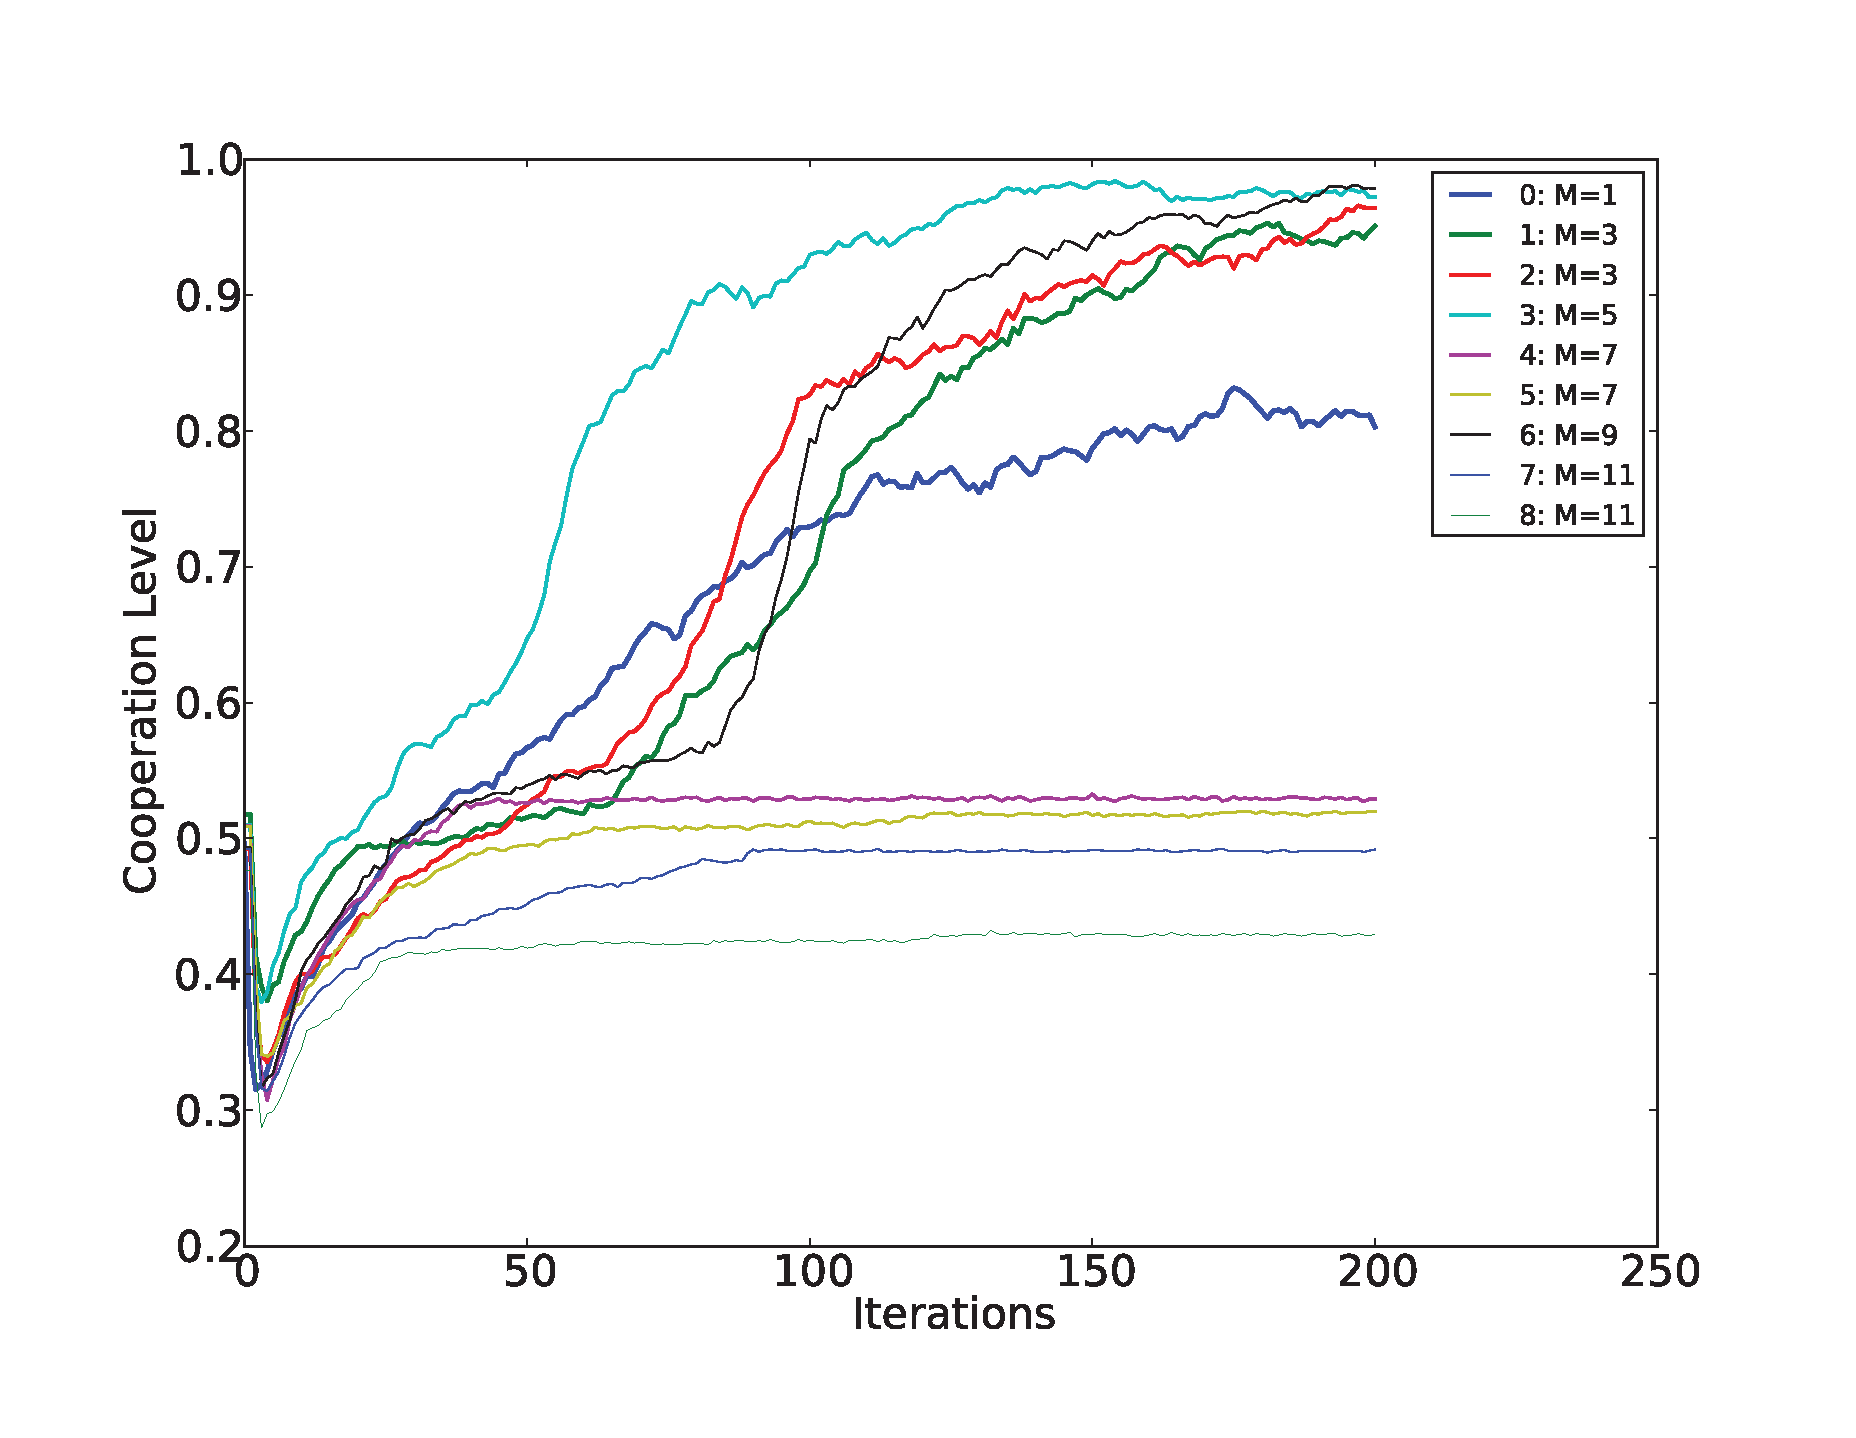
\includegraphics[width=12cm]{../figures/configurations_d09_s0.eps}}
\caption{Evolution of cooperation for $d=0.9$, with $M = \{1,3,5,7,9,11\}$. Cooperation does best for medium migration ranges $M = \{ 3,5\}$. For $M \geqslant 7$, cooperation is stuck between 40\% and 55\%, at the notable exception of $M=9$, which performs as well as $M = \{ 3,5\}$. It looks like that, for all $M$, cooperators counter defector invasion by creating small clusters, which grow up to a saturation where these clusters can survive surrounded by defectors. In some cases $M = \{ 3,5,9\}$, cooperators manage to unlock the situation and further break the belt of defectors. {\bf [The conditions for this to happen remain unclear to me so far, especially that $M=9$ performs like $M = \{ 3,5\}$ rather than like $M = \{ 7,11\}$]}.}
\label{fig:medium_d_migration}
\end{center}
\end{figure}



We shall study in more details the origins of this chaotic behavior, leading either to  $0.4 \leqslant c \leqslant 0.6$ after $t=200$ iterations or to $ c > 0.9$. We inspect how migration patterns in the latter case, influence departure from the former dynamics.\\

\begin{figure}[H]
\begin{center}
\centerline{\includegraphics[width=13cm]{../figures/configuration_d09_s0.eps}}
\caption{Effects of migration in densely populated grids ($d=0.9$). With small migration range $M=1$ (see {\bf B.}), clusters of cooperators form quickly, along with defectors around these clusters. The small migration range does not allow cooperators to jump over defectors. When the migration range is larger $M=5$ (see {\bf C.}), similar clusters of cooperators form at first ($t = 35$), but the larger migration range allows creating connected clusters ($t = 56$), which in turn help overcome most defectors ($t = 200$).}
\label{fig:high_d_migration}
\end{center}
\end{figure}



%\begin{figure}[H]
%\begin{center}
%%\centerline{\includegraphics[width=13cm]{../figures/configuration_d09_s0.eps}}
%\caption{Here a comparison of between a normally continuing simulation, and a sudden drop after $t = 150$ iterations (c.f. time series plots). The hope here is to find a (qualitative) pattern change between these two configurations, which may predict the drop of cooperators.}
%\label{fig:sudden_regime_change}
%\end{center}
%\end{figure}


\clearpage

\subsection*{Migration and Property Games in Medium Populated Worlds ($0.4 \leqslant d \leqslant 6$)}

{\bf [Some text here]}

\begin{figure}[H]
\begin{center}
\centerline{\includegraphics[width=14cm]{../figures/TimeSeriesPhaseTransitions.eps}}
\caption{Evolution of cooperation for average grid density $0.40 \leqslant d < 0.60$ over $N=200$ iterations for migration ranges $M = \{ 1,3,5,7,9,11,13\}$ and for property violation values $s$ close to $s^*(M)$ (migration probability $m=1$). The presented time series illustrate how the property violation phase transition occurs as a function of the migration range. Populations with a small migration range $M=1$ can enhance cooperation after an initial drop. Yet little migration capabilities, make populations very sensitive to property violation: for $s^{*} > 0.05$, defectors win quickly (see {\it A.}). For $M=5$, we observe two scenarios regarding property violation: Either cooperative populations win $s < s^{*} = 0.158$ or on the contrary, they disappear for $s>s^{*}$. It appears that populations, which cannot a sustain a cooperation level higher than $0.5$, almost surely defect  (see {\it B.}). As migration range gets larger ($M = \{7,9\}$), an intermediary state appears, in which populations can sustain clusters of cooperation for some time, while defectors are in majority (see {\it C.} and {\it  D.}). For even larger migration ranges ($M = \{11,13\}$), this intermediary state appears even more clearly (see {\it E.} and {\it  F.}), with cooperative populations in minority ($c \approx 0.45$ for $M=11$ and $c \approx 0.40$ for $M=13$), yet clustered in a world of defectors (see Figure \ref{fig:configurations_t200_M11plus} {\it C} and {\it G}).}
\label{fig:tseries_phase_transition}
\end{center}
\end{figure}


%\begin{figure}[H]
%\begin{center}
%\centerline{\includegraphics[width=13cm]{../figures/configuration_d05_s0.eps}}
%\caption{}
%\label{fig:medium_d_migration}
%\end{center}
%\end{figure}


\begin{figure}[H]
\begin{center}
\centerline{\includegraphics[width=13cm]{../figures/configuration_d05_s0.eps}}
\caption{}
\label{fig:medium_d_migration}
\end{center}
\end{figure}



\end{document}

